% Sources: data/raw/README.md, CASES.csv, DATA_DICTIONARY.csv;
% results/audit/report.md, quality_summary.json and tables/.
% Four context slides followed by the preprocessing-results subsection.
\section{Input Data}

\begin{frame}[more-space]{Input Data\enspace|\enspace Operating cases and model variables}
  \begin{columns}[T,onlytextwidth]
    \column{0.47\textwidth}
      \dataheading{Measured variables}
      {\footnotesize
      \renewcommand{\arraystretch}{1.25}
      \setlength{\tabcolsep}{4pt}
      \begin{tabular*}{\linewidth}{@{\extracolsep{\fill}}lr@{}}
        \toprule
        \textbf{Model input} & \textbf{Observed range}\\
        \midrule
        Total CPU power & 329--2,312 W\\
        Inlet air temperature & 23.4--46.4\,${}^\circ$C\\
        Raw fan signal & 0.117--0.766\\
        \midrule
        \textbf{Response} & \\
        Maximum CPU temperature & 36--95\,${}^\circ$C\\
        \bottomrule
      \end{tabular*}
      \smallskip
      Marginal ranges include transition rows.\\
      Fan signal: original scale, unit unverified.
      }

    \column{0.50\textwidth}
      \dataheading{Five operating regimes}
      {\footnotesize
      \renewcommand{\arraystretch}{1.12}
      \setlength{\tabcolsep}{4pt}
      \begin{tabular*}{\linewidth}{@{\extracolsep{\fill}}lrrr@{}}
        \toprule
        \textbf{Case} & \textbf{Inlet} & \textbf{DP} & \textbf{Rows}\\
        & $[{}^\circ\mathrm{C}]$ & $[\mathrm{kPa}]$ & \\
        \midrule
        \casekey{caseone}{1}   & 25 &  2 & 249\\
        \casekey{casetwo}{2}   & 35 &  4 & 304\\
        \casekey{casethree}{3} & 45 &  6 & 237\\
        \casekey{casefour}{4}  & 45 &  8 & 309\\
        \casekey{casefive}{5}  & 45 & 10 & 209\\
        \bottomrule
      \end{tabular*}
      \smallskip
      Inlet and DP: \textbf{setpoints}; DP $\ne$ fan power.\\
      \texttt{stress-ng}: \textbf{100 / 75 / 50 / 25\,\% / idle}\\
      Case labels: curated constant-setpoint stretches
      }
  \end{columns}

  \medskip
  \begin{beamercolorbox}[sep=1.3mm,wd=\textwidth]{data panel}
    \footnotesize
    \textbf{Modeling subset}\quad Select steady-state intervals; curated case labels alone are insufficient.\\
    \textbf{Strict maximum}\quad All CPU temperature readings required; no missing-sensor imputation.
  \end{beamercolorbox}

  \datasource{Sources: CASES.csv; results/audit/report.md, case\_summary.csv and numerical\_ranges.csv.
    Marginal ranges describe observations, not a fully tested operating box.}
\end{frame}

\subsection{Problems with the dataset}

\begin{frame}[more-space]{Input Data\enspace|\enspace Problems with the dataset}
  \begin{columns}[T,onlytextwidth]
    \column{0.46\textwidth}
      \dataheading{Observed inlet / fan combinations}
      \centering
      % Panel (a) of the existing vector figure; other panels and the shared
      % legend are clipped only at display time. Source PDF stays unchanged.
      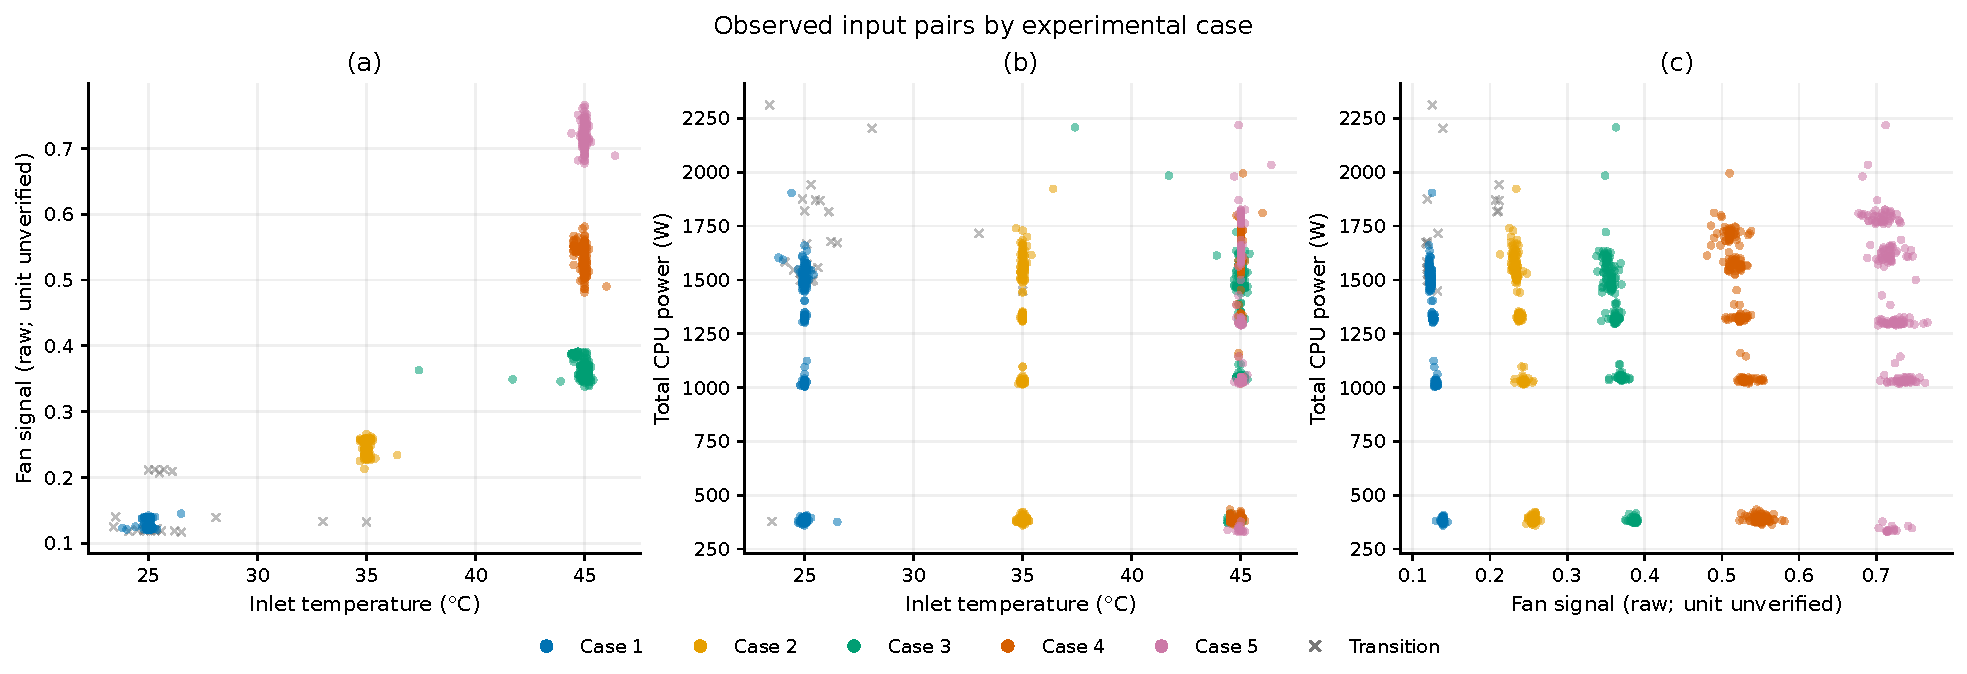
\includegraphics[width=\linewidth,height=49mm,keepaspectratio,
        trim=0bp 24bp 634bp 40bp,clip]
        {../../results/audit/figures/pairwise_input_scatter.pdf}
      \par\smallskip
      {\footnotesize
        \casekey{caseone}{1}\quad\casekey{casetwo}{2}\quad
        \casekey{casethree}{3}\quad\casekey{casefour}{4}\quad
        \casekey{casefive}{5}\quad{\color{black!50}$\times$}\,transition
      }

    \column{0.51\textwidth}
      \begin{beamercolorbox}[sep=2mm,wd=\linewidth]{data panel}
        \dataheading{1. Sparsity}
        {\large\color{rwth-blue-100}\bfseries 31 / 125}\;occupied grid cells\par
        \smallskip
        Five bins per input; binning-dependent diagnostic\\
        Five trajectories; no full factorial design\\
        \textbf{Untested:} high fan signal at $25\,{}^\circ$C
      \end{beamercolorbox}

      \medskip
      \begin{beamercolorbox}[sep=2mm,wd=\linewidth]{data warning}
        \dataheading{2. Unverified unit of fan signal}
        Dictionary confidence: \textbf{low}\\
        Retain raw scale; no W / kW conversion\\
        Calibrated fan-energy costs unavailable\\
        \textbf{Needed:} confirmation from data owners
      \end{beamercolorbox}

      \medskip
      {\footnotesize\textbf{Modeling:} validate new combinations before optimization.}
  \end{columns}

  \datasource{Sources: exploratory audit, coverage\_grid.csv and DATA\_DICTIONARY.csv.
    Figure: pairwise\_input\_scatter.pdf (a). Grid occupancy: labeled cases only;
    resolution-dependent diagnostic, not a validated operating boundary.}
\end{frame}

\begin{frame}[more-space]{Input Data\enspace|\enspace Problems with the dataset}
  \begin{columns}[T,onlytextwidth]
    \column{0.66\textwidth}
      \dataheading{Observed correlations between the model inputs}
      % Use the existing vector figure in place; trim its redundant top title.
      % Both correlation matrices, tick labels, and the color scale are retained.
      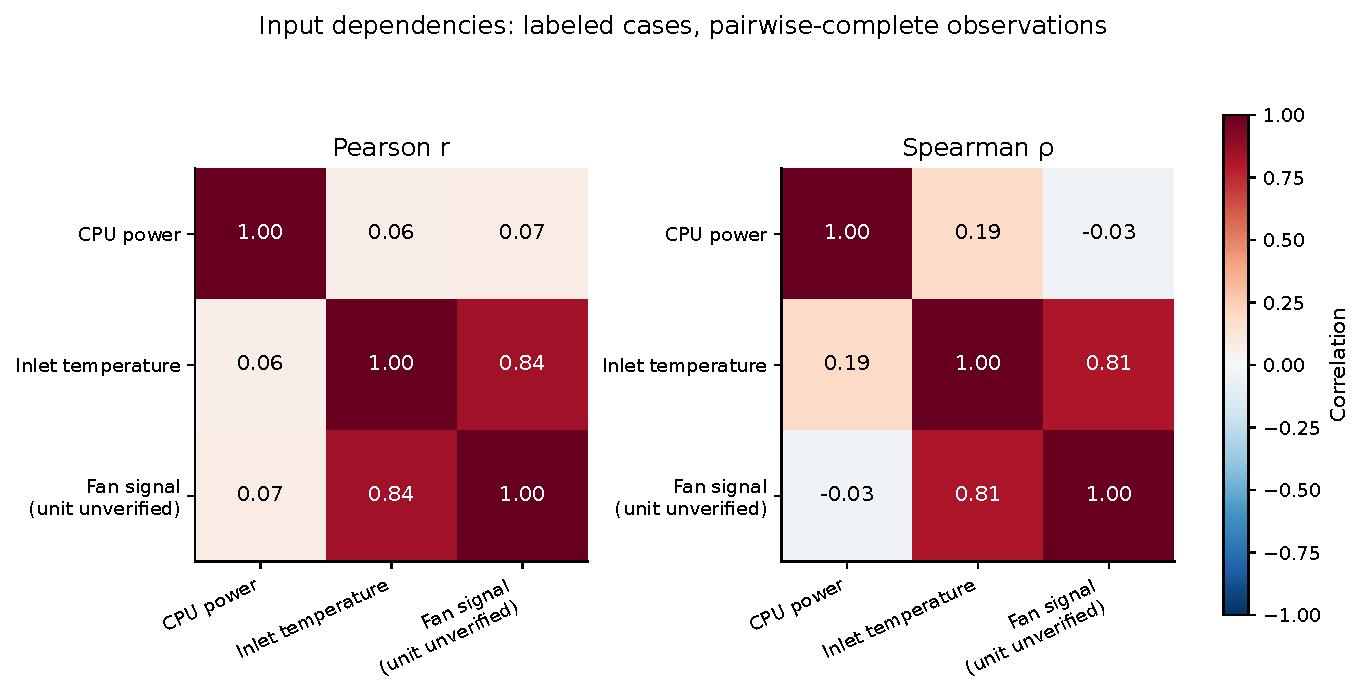
\includegraphics[width=\linewidth,trim=0bp 0bp 0bp 35bp,clip]
        {../../results/audit/figures/input_correlation_matrix.pdf}
      \par\smallskip
      {\footnotesize
        Pearson: linear / Spearman: rank correlation\\
        Labeled cases 1--5; pairwise-complete observations ($n=1{,}308$)
      }

    \column{0.31\textwidth}
      \begin{beamercolorbox}[sep=2mm,wd=\linewidth]{data panel}
        \dataheading{3. Input Dependence}
        \textbf{Fan signal / inlet temperature}\par
        \smallskip
        {\large\color{rwth-blue-100}\bfseries $r=0.84$\quad $\rho=0.81$}\par
        \smallskip
        Shared experimental case design\\
        Strong pooled association
      \end{beamercolorbox}

      \medskip
      \dataheading{Implications for PCE / UQ}
      \footnotesize
      Independent marginal sampling\\
      $\rightarrow$ untested input combinations

      \medskip
      Review independence assumptions\\
      before classical PCE / Sobol analysis

      \medskip
      \textbf{Near-zero correlation}\\
      $\ne$ statistical independence
  \end{columns}

  \datasource{Sources: results/audit/report.md and tables/input\_dependencies.csv.
    Figure: input\_correlation\_matrix.pdf, referenced directly from results/audit/figures/.
    Pooled relationships include between-case changes; correlation does not establish causality.}
\end{frame}

\subsection{Need for preprocessing and steady-stateness of the data}

\begin{frame}[more-space]{Input Data\enspace|\enspace Need for preprocessing and steady-stateness of the data}
  \begin{columns}[T,onlytextwidth]
    \column{0.56\textwidth}
      \dataheading{Load steps and thermal response}
      % Display panels (a) and (d) from the same existing time-series PDF.
      % The shared case colors and time axis are retained; no data are altered.
      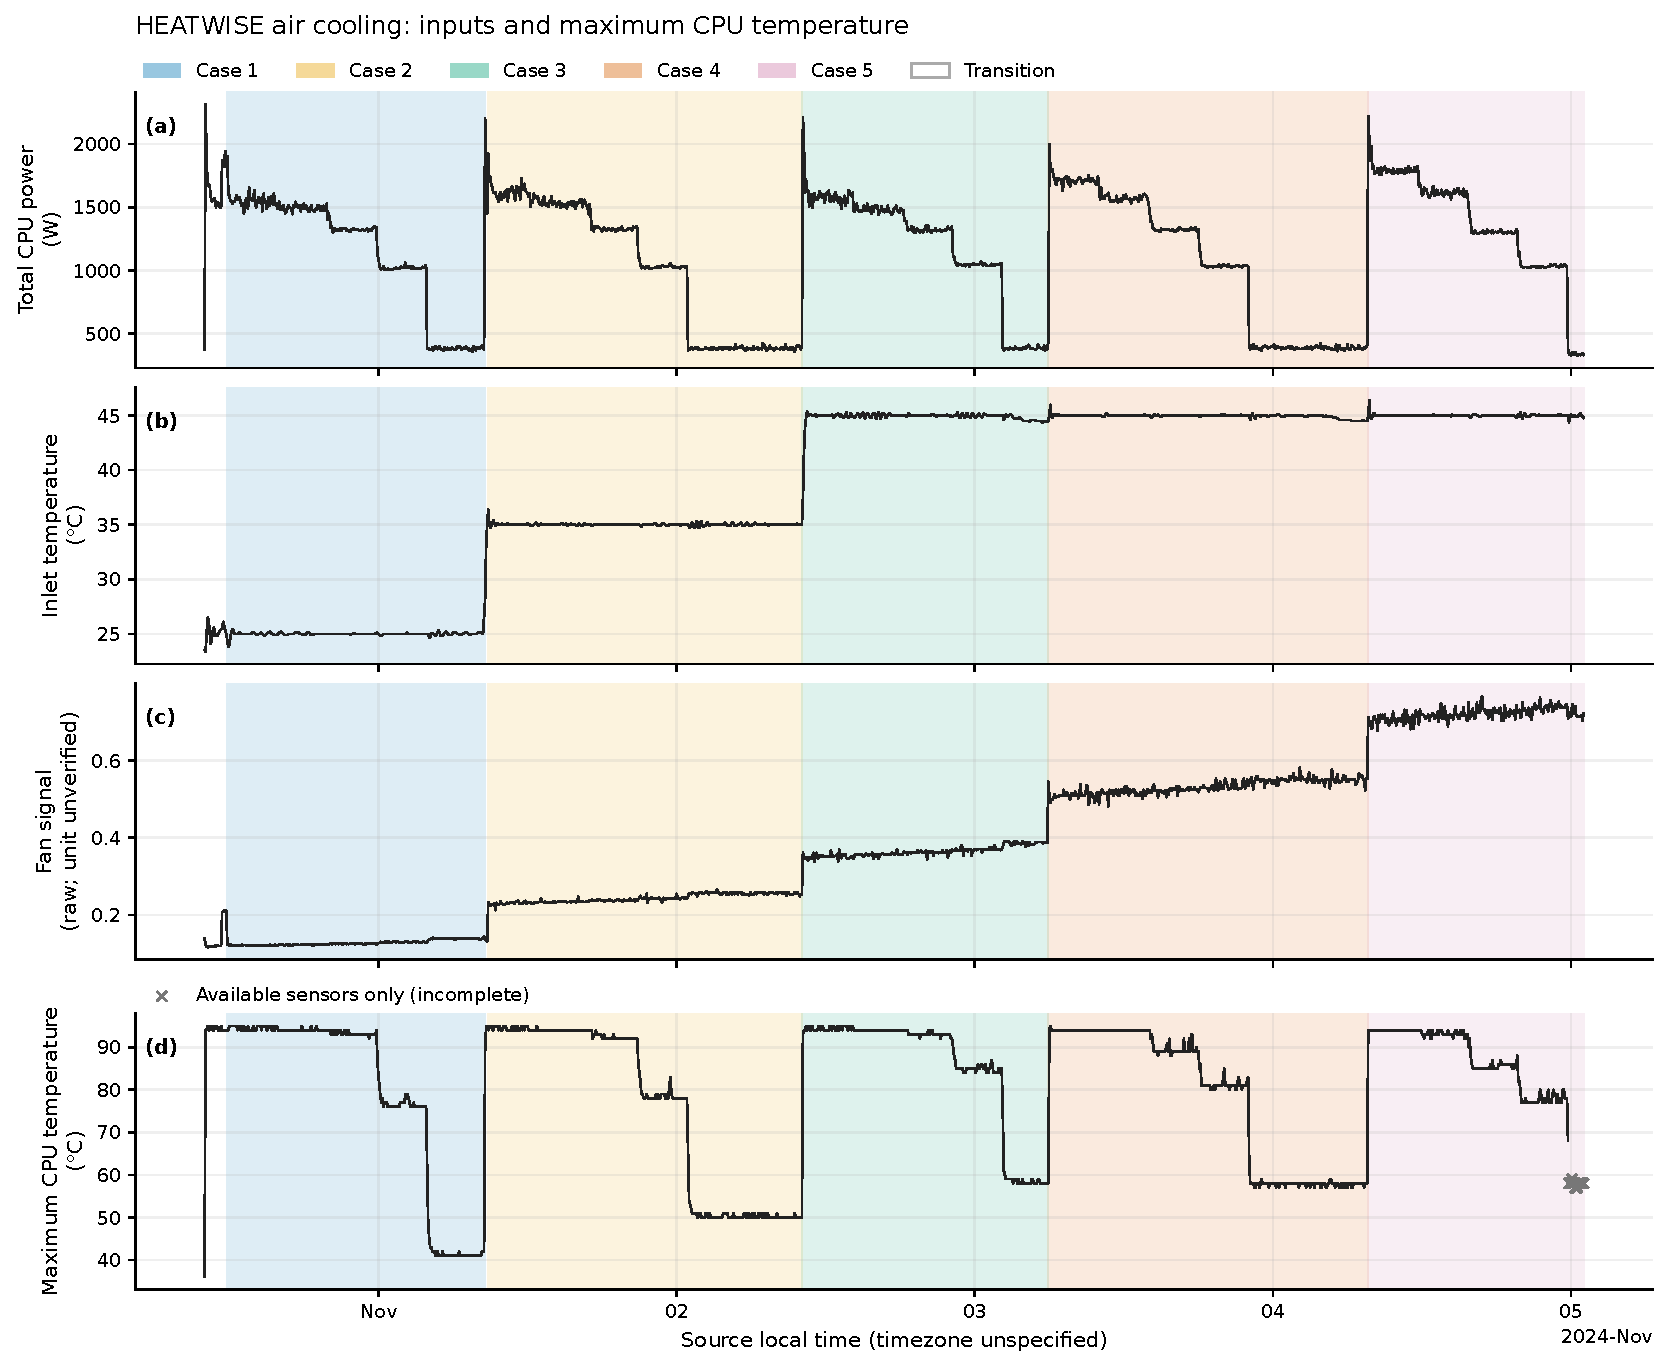
\includegraphics[width=\linewidth,trim=0bp 478bp 0bp 22bp,clip]
        {../../results/audit/figures/inputs_and_max_temperature_timeseries.pdf}
      \par\vspace{1mm}
      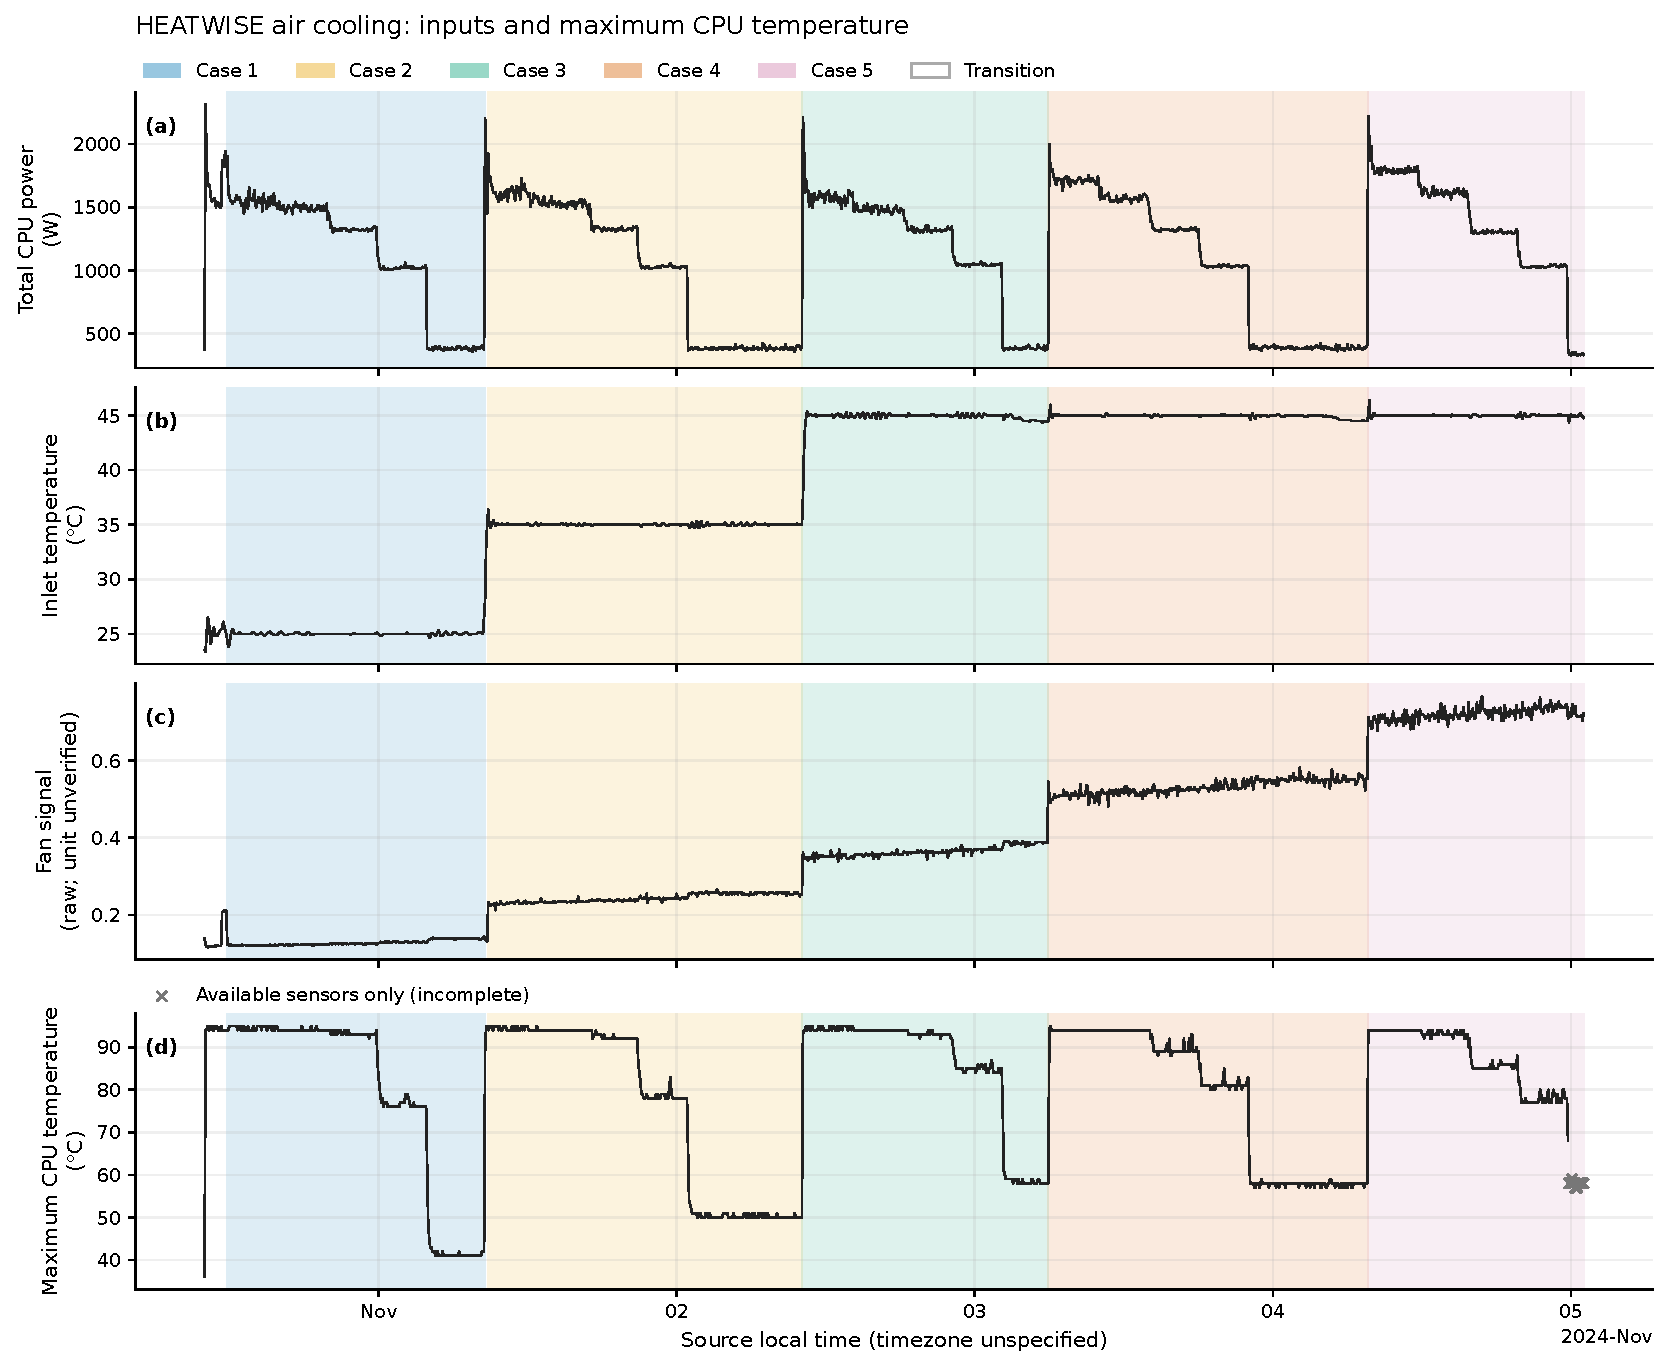
\includegraphics[width=\linewidth,trim=0bp 0bp 0bp 472bp,clip]
        {../../results/audit/figures/inputs_and_max_temperature_timeseries.pdf}
      \par\medskip
      {\footnotesize
        \textbf{25} unlabeled start-up / transition rows\\
        \textbf{15} rows with incomplete CPU readings\\
        Strict $T_{\max}$: all 18 sensors required
      }

    \column{0.41\textwidth}
      \begin{beamercolorbox}[sep=2mm,wd=\linewidth]{data panel}
        \dataheading{Preprocessing before fitting}
        \footnotesize
        Separate start-up / transition rows\\
        Flag incomplete CPU temperature readings\\
        Derive strict maxima from complete sensor sets\\
        Preserve raw data; no sensor imputation
      \end{beamercolorbox}

      \medskip
      \begin{beamercolorbox}[sep=2mm,wd=\linewidth]{data panel}
        \dataheading{Select steady-state intervals}
        \footnotesize
        Case label $\ne$ thermal equilibrium\\
        Exclude settling after load / setpoint changes\\
        Stable inputs \textbf{and} CPU temperatures\\
        Paper: $\geq 10$ min steady-state averages\\
        Five-minute sampling / averaging: unclear
      \end{beamercolorbox}
  \end{columns}

  \datasource{Sources: data/raw/README.md; results/audit/report.md and quality\_summary.json.
    Figure: inputs\_and\_max\_temperature\_timeseries.pdf, panels (a) and (d). Implemented selection and results follow.}
\end{frame}

% Existing selection figure is included directly, without changing data.
\subsection{Preprocessing results}
\definecolor{selectiongreen}{HTML}{009E73}

\begin{frame}[more-space]{Input Data\enspace|\enspace Preprocessing results}
  \begin{columns}[T,onlytextwidth]
    \column{0.56\textwidth}
      \dataheading{Selected approximately steady intervals}
      \centering
      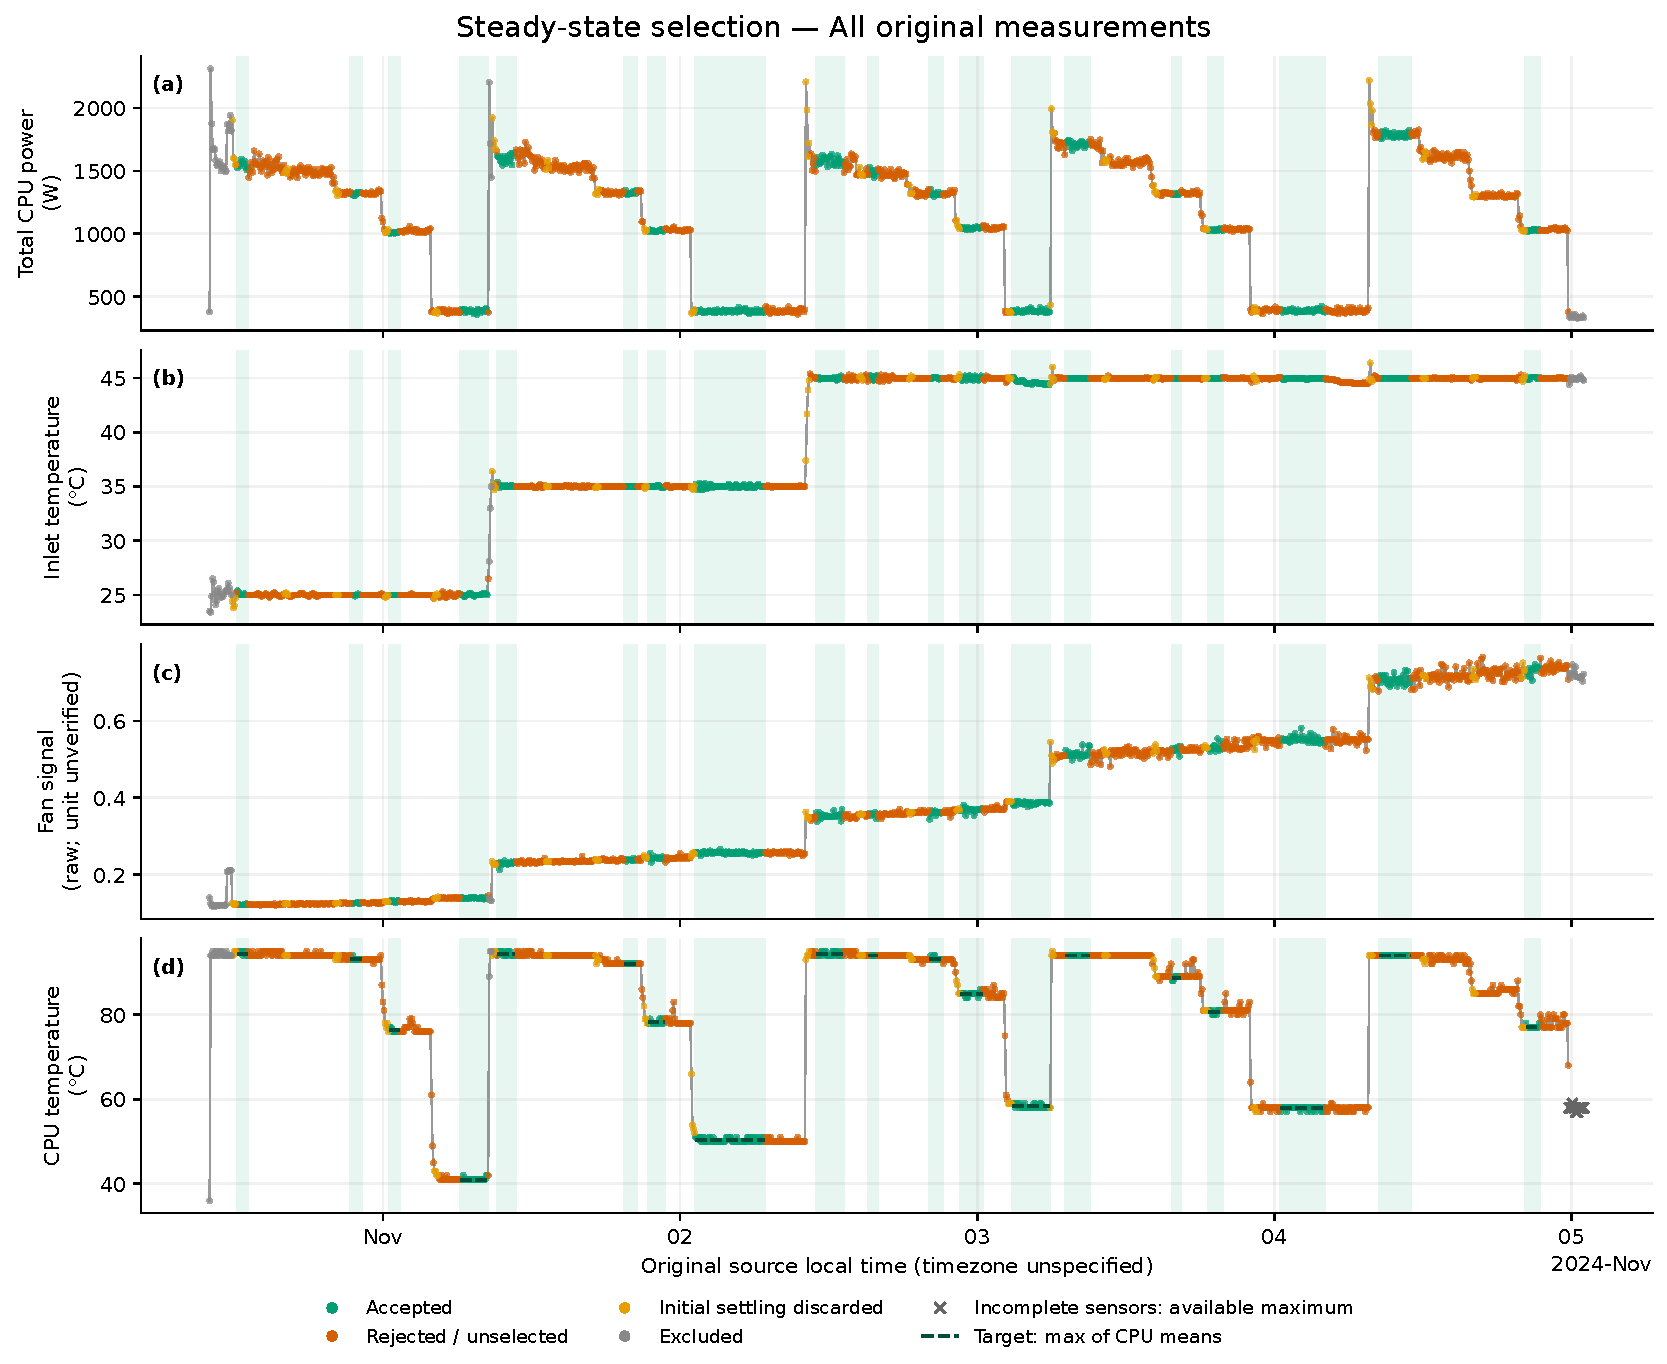
\includegraphics[width=\linewidth,height=50mm,keepaspectratio]
        {../../results/preprocessing/figures/selection_overview.pdf}
      \par\smallskip
      {\small\color{selectiongreen}\textbf{One green band = one processed observation.}}
      \par\smallskip
      {\footnotesize \textbf{60-minute dwell: 14 observations} (backup).}

    \column{0.41\textwidth}
      \begin{beamercolorbox}[sep=2mm,wd=\linewidth]{data panel}
        {\color{rwth-blue-100}\fontsize{22}{25}\selectfont\bfseries 19}\par
        \textbf{operating observations}\par
      \end{beamercolorbox}
      \medskip
      \dataheading{Each observation contains:}
      \footnotesize
      \[
        \Bigl(
          \underbrace{\bar P_{\mathrm{CPU}},\,\bar T_{\mathrm{inlet}},\,\bar F}_{\text{three inputs}},\;
          \underbrace{\max_{j=1,\ldots,18}\bar T_j}_{\text{temperature target}}
        \Bigr)
      \]
      Interval averages; $j=1,\ldots,18$ indexes CPUs.
      \par\smallskip
      \begin{beamercolorbox}[sep=1.5mm,wd=\linewidth]{data warning}
        \dataheading{Our starting choice: degrees 1 and 2}
        \footnotesize
        \begin{itemize}
          \item Full bases: \textbf{4 / 10 coefficients}; cubic: 20 ($>19$).
          \item Quadratic design: $\kappa_2\approx702$; coefficients may be unstable.
          \item Higher degrees need sparsity / regularization; validate either choice.
        \end{itemize}
      \end{beamercolorbox}
  \end{columns}
\end{frame}

% Assumed reference distributions; experimental data are unchanged.
\subsection{Input distributions}

\begin{frame}[more-space]{Input Data\enspace|\enspace Input distributions}
  \dataheading{Uniform inputs: equal weight across each observed range}
  \small
  Bounds come from the \textbf{19 processed observations}.
  \par\medskip
  {\renewcommand{\arraystretch}{1.35}
  \begin{tabular*}{\textwidth}{@{\extracolsep{\fill}}lrrl@{}}
    \toprule
    \textbf{Input} & \textbf{Lower bound} & \textbf{Upper bound} & \textbf{Unit}\\
    \midrule
    Total CPU power & 384.735 & 1,786.226 & W\\
    Inlet air temperature & 25.000 & 45.056 & ${}^\circ$C\\
    Raw fan signal & 0.121636 & 0.730571 & unverified\\
    \bottomrule
  \end{tabular*}}
  \smallskip
  \begin{beamercolorbox}[sep=1.5mm,wd=\textwidth]{data panel}
    \dataheading{Scale each parameter to $[-1,1]$}
    \footnotesize
    \setlength{\abovedisplayskip}{2pt}
    \setlength{\belowdisplayskip}{2pt}
    \[
      x_i\in[a_i,b_i]\quad\Longrightarrow\quad
      \xi_i=2\frac{x_i-a_i}{b_i-a_i}-1
    \]
    Lower bound $\mapsto-1$; midpoint $\mapsto0$; upper bound $\mapsto1$.\par
    Uniform reference inputs become $\mathcal U(-1,1)$: Use a normalized \textbf{Legendre} basis as the orthonormal polynomial family for the PCE.
  \end{beamercolorbox}
\end{frame}

\subsection{Digital Twin Definition}

\begin{frame}[more-space]{Summary: Digital Twin Definition}
  {\normalfont\small
  \renewcommand{\arraystretch}{1.35}
  \setlength{\tabcolsep}{4pt}
  \begin{tabular}{@{}p{0.23\textwidth}p{0.73\textwidth}@{}}
    \toprule
    \textbf{Element} & \textbf{Our thermal digital twin}\\
    \midrule
    \textbf{Model} & \mdseries
      Planned: PCE vs PI-PCE with monotonicity constraints; degrees 1 / 2\\
    \midrule
    \textbf{Parameters} & \mdseries
      Surrogate coordinates: CPU power $P$, fan signal $F$, inlet temperature $T$\\
    \midrule
    \textbf{Inputs} & \mdseries
      Surrogate: $(P,T,F)$; controller disturbance: inlet temperature\\
    \midrule
    \textbf{Outputs} & \mdseries
      Surrogate: maximum interval-mean CPU temperature; controller: proposed $(P,F)$\\
    \midrule
    \textbf{Measurement operator} & \mdseries
      18 CPU sensors, every 5 min; $\mathcal H=\max_{j=1,\ldots,18}\overline{T}_j$ over an approximately steady period\\
    \midrule
    \textbf{Observables} & \mdseries
      19 approximately steady temperature targets\\
    \midrule
    \textbf{Quantity of interest} & \mdseries
      CPU / fan choice within a validated domain and error bound; hardware protects peaks\\
    \bottomrule
  \end{tabular}
  }
\end{frame}

